\newpage
\section{Aufbau des neuronalen Netzes}

In diesem Abschnitt wird erklärt, wie unser neuronales Netz aufgebaut ist. Vor allem die Abbildung \ref{AnordungMerkuPix} ist für das bessere Verständnis der Matlab-Skripte wichtig. In den Matlab-Skripten, welche unter anderem im \ref{Appendix} zu finden sind, muss immer die Pixelanzahl pro Merkmal (in Abbildung \ref{AnordungMerkuPix} N) wie auch die Anzahl der Merkmale (in Abbildung \ref{AnordungMerkuPix} M) angegeben werden. Dabei handelt es sich immer um einen symmetrischen Aufbau. Ist die Merkmalanzahl gleich 5, dann gibt es 25 Merkmale (5 in x-Richtung und 5 in y-Richtung). Das gleiche gilt für die Pixelanzahl. Bei einer Pixelanzahl von 8 werden für jedes Merkmal so 64 Pixel angenommen. Bei einer Merkmalanzahl von 5 und einer Pixelanzahl von 8 wird also eine Pixelmatrix von 40 mal 40 Pixel erzeugt und jeweils anhand der Merkmale behandelt.

\begin{figure}[hbt]
	\centering
	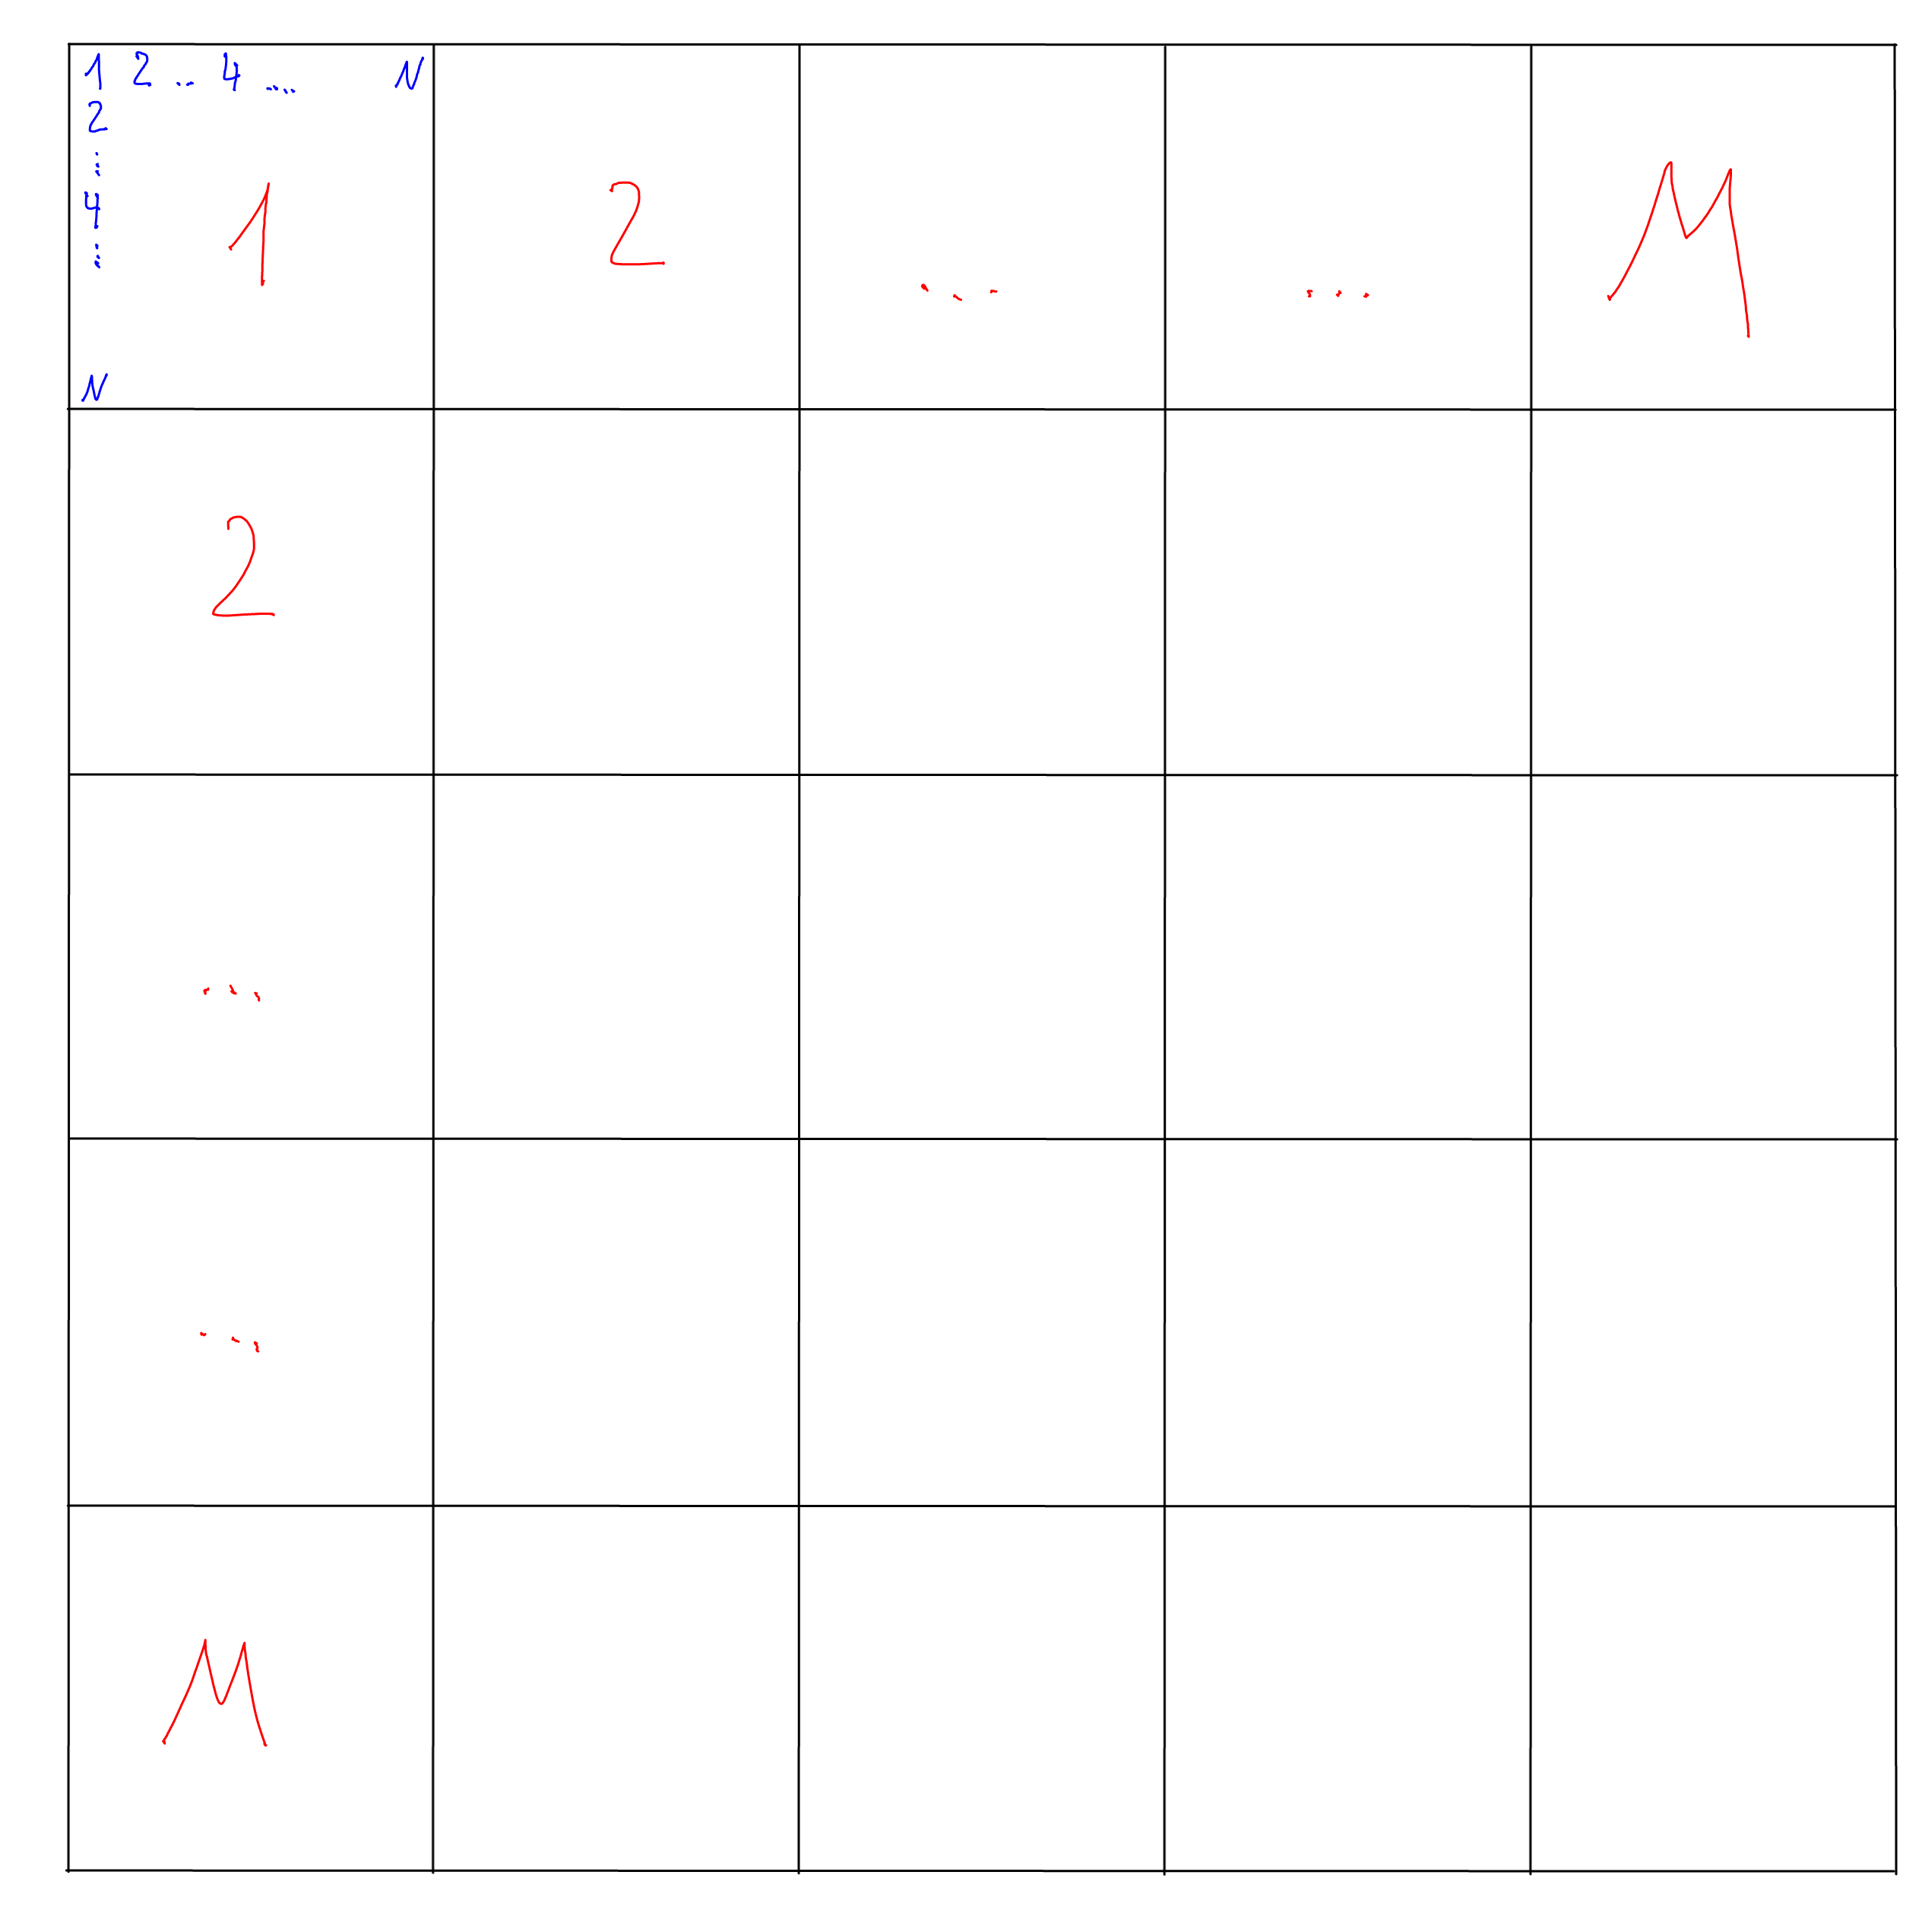
\includegraphics[width=0.8\linewidth]{./Bilder/Auswertung/Aufbau/page4}
	\caption{Anordnung der Merkmale und Pixel}
	\label{AnordungMerkuPix}
\end{figure}

In Abbildung \ref{Neuron1Ebene} ist ein beispielhaftes Neuron abgebildet. Dieses Neuron der 1. Ebene fasst ein komplettes Merkmal mit all seinen Pixeln zusammen. Es verfügt also in unserem Beispiel über 64 Eingänge und es gibt 25 dieser Neuronen in der ersten Ebene des Netzes.

\begin{figure}[hbt]
	\centering
	
\includegraphics[width=0.8\linewidth]{./Bilder/Auswertung/Aufbau/page5}
	\caption{Neuron der 1. Ebene}
	\label{Neuron1Ebene}
\end{figure}

Mit einer einzigen Ebene von Neuronen kann bereits viel erreicht werden. Allerdings ist für die Gesamtauswertung eine zweite Ebene von Vorteil, um zum Beispiel bei starkem Rauschen Fehler besser zu detektieren. Bevor wir die zweite Ebene der Neuronen betrachten, werfen wir einen Blick auf die Abbildung \ref{Erl2Ebene}. Hier sind drei Arten von Merkmalen zu erkennen. Die fünf schwarz hervorgehobenen Merkmale detektieren einen horizontalen Balken, die blauen hervorgehobenen einen vertikalen Balken und die roten Merkmale können ein hohes Rauschen beziehungsweise auch zur Detektion von Fehlern ausgewertet werden. Die roten Merkmale erlauben es, eine bessere Konfiguration des neuronalen Netzes zu finden. Durch die Kombination der blau wie auch der schwarz hervorgehobenen Merkmale ergibt somit zusätzlich die Möglichkeit ein Kreuz zu detektieren.

\begin{figure}[hbt]
	\centering
	\includegraphics[width=0.5\linewidth]{./Bilder/Auswertung/Aufbau/Merkmal-Aufteilung}
	\caption{Erläuterung der Anordnung für die 2. Ebene}
	\label{Erl2Ebene}
\end{figure}

In Abbildung \ref{Neurin2Ebene} ist die zweite Ebene des Neuronalen Netzes dargestellt. Die Ausgänge der einzelnen Merkmale dienen anhand ihres jeweiligen Merkmaltyps den Neuronen der zweiten Ebene als Input. In diesem Fall sind alle Gewichte auf eins gesetzt. Es wird lediglich der Bias eingestellt und somit die Schwelle zur Detektion festgelegt. 

\begin{figure}[hbt]
	\centering
	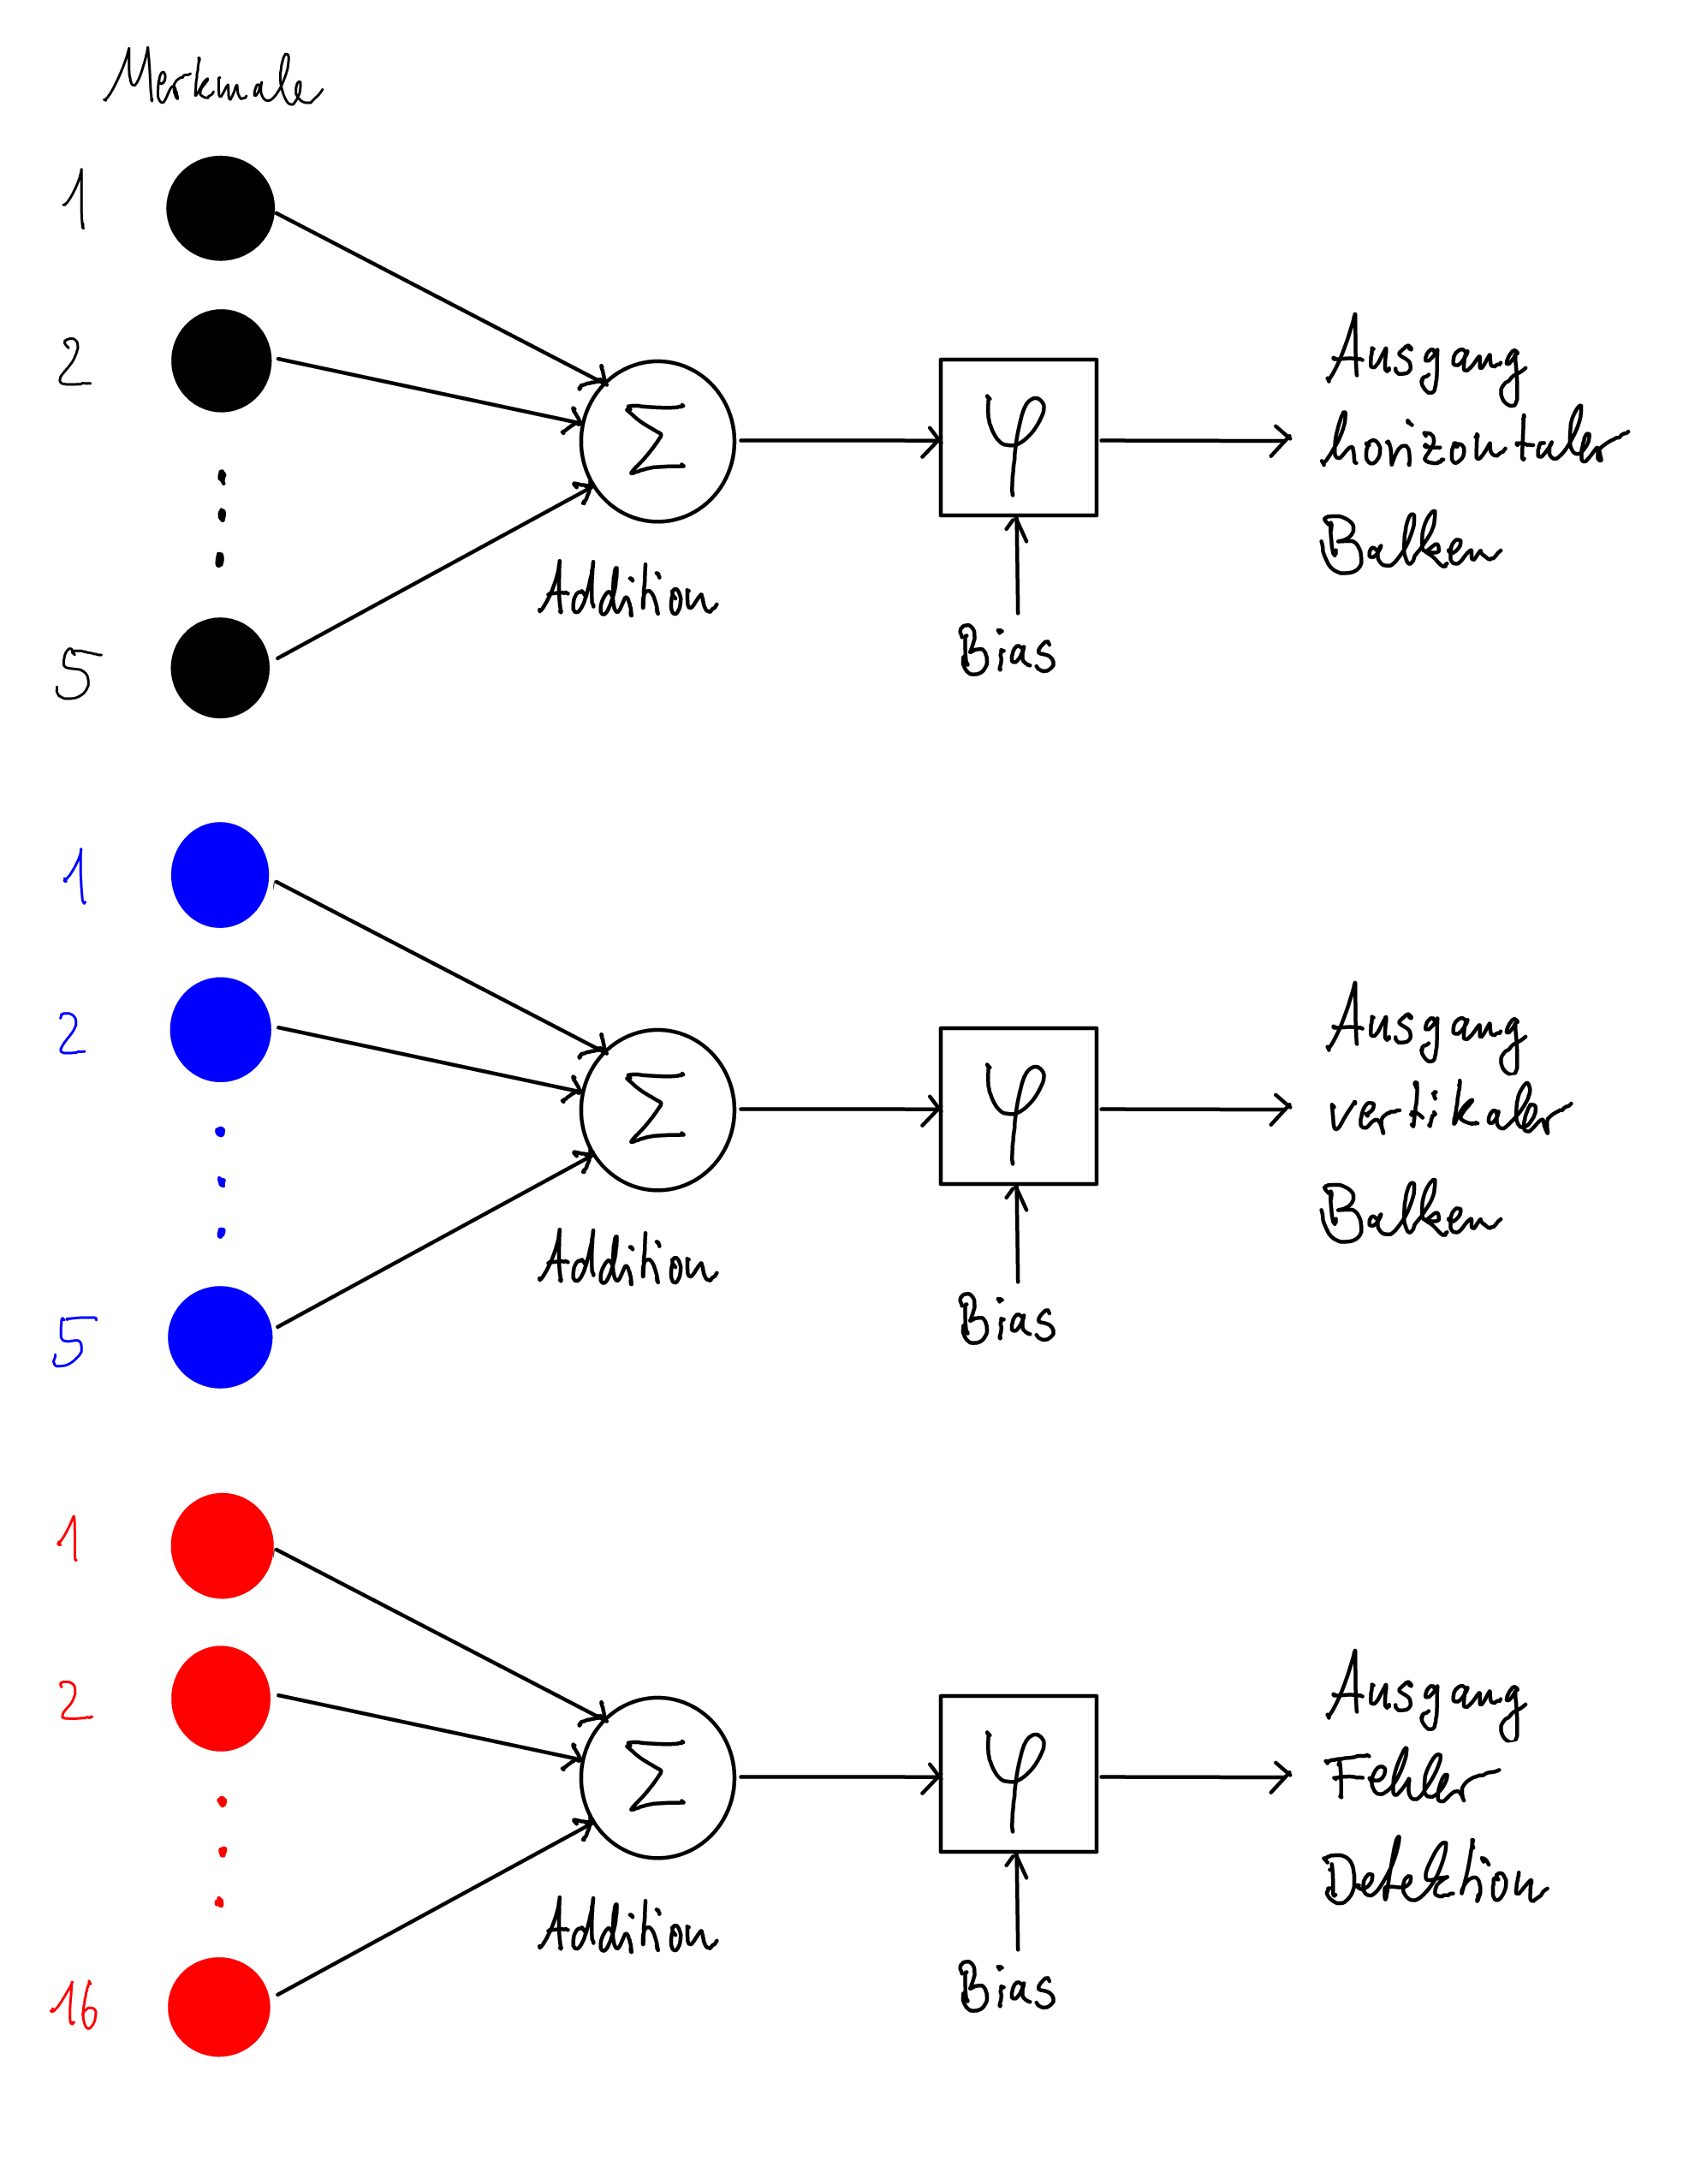
\includegraphics[width=0.8\linewidth]{./Bilder/Auswertung/Aufbau/page7}
	\caption{Neuronen der 2. Ebene}
	\label{Neurin2Ebene}
\end{figure}

Für die Auswertung der Neuronen der erste Ebene nutzen wir eine Sigmoid-Funktion. Für die zweite Ebene werden die addierten Werte werden ohne eine weiteren Verarbeitung weiter gegeben. Das entspricht einer linearen Aktivierungsfunktion mit dem Anstieg eins.
